\subsection{Collaboration diagram}

\begin{figure}[h]
\centering
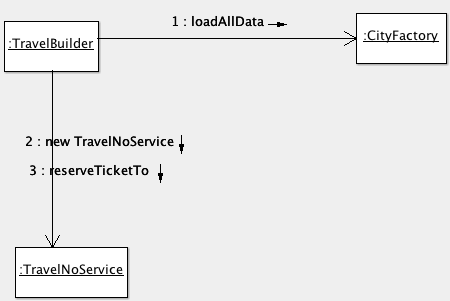
\includegraphics[width=12cm]{project/images/collaboration.png}
\caption{Collaboration diagram}
\end{figure}

\paragraph{}
To create a reservation without service, an instance of class \textit{TravelNoService}, we need three steps. 

\begin{itemize}
\item A factory need to load all data from file.
\item TravelBuilder create an instance of \textit{TravelNoService}. No specified data yet.
\item TravelBuilder request this instance to use method \textit{reserveTicketTo} to make a flight reservation, then return the instance.
\end{itemize}